%datadasedesign.tex
The database is designed in MySQL 5.1.61, and resembles the local database created by Oasis -- the only difference is, that the Savannah database has two extra attributes in the \code{AuthUsers} table: \code{username} and \code{password}. The reason for this is that while all GIRAF apps running on the Android platform uses QR-codes for user authentication, this is not a feasible solution for the web interface, as it can not be assumed that every user has a webcam conneceted to the computer.

\subsubsection{Requirements}
\label{subsec:databaseReq}
The requirements for the database has been provided by the other project groups, and are as follows:

\begin{itemize} % TODO ohnoes..punktummer
	\item All users must be able to login with a QR-code
	\item Each department must also be able to login
	\item All users must be linked to at least one department
	\item All guardians must be able to be linked to at least one child.
	\item All parents must be able to be linked to at least one child.
	\item All users must be able to have to their selected apps
	\item All users must be able to access their own pictures, and all public pictures
	\item All departments must be able to access all public pictures
	\item All pictures needs to be able to be linked to tags
	\item Pictures must be able to be linked with audio and vice versa
	\item A department must be able to have a subdepartment\footnote{Example: Birken has two departments, at two different addresses, both these subdepartments needs to be linked with Birken as a superdepartment}
\end{itemize}

\subsubsection*{Early Diagrams}
The database has had several redesigns, due to new demands and new ideas.
\begin{description}
	\item[First draft (0.2)] The first draft of the database can be seen in \autoref{fig:draft02}. There were several missing fields in this draft: username and password is missing form the \code{AuthUsers}, and department has no access to \code{Media}, 
	\item[Second draft (0.3)] The second draft of the database can be seen in \autoref{fig:draft03}. This handles the problem of a department's access to medias.
	\item[Third draft (0.4.1)] Several tables has been renamed to ease understanding.
	\item[Final draft] The final database can be seen in \autoref{fig:DiaDesign}. This handles the problem with username and password in the \code{AuthUsers}, departments access to medias, and proper naming of both tables and attributes.
\end{description}

\subsubsection*{Current Database} %TODO fix overskrift
A diagram has been made to get a overview of the different tables and their relations. This diagram is designed in DIA\cite{Dia}, and can be seen in \autoref{fig:DiaDesign}.

\begin{figure}[htbp]
	\centering
		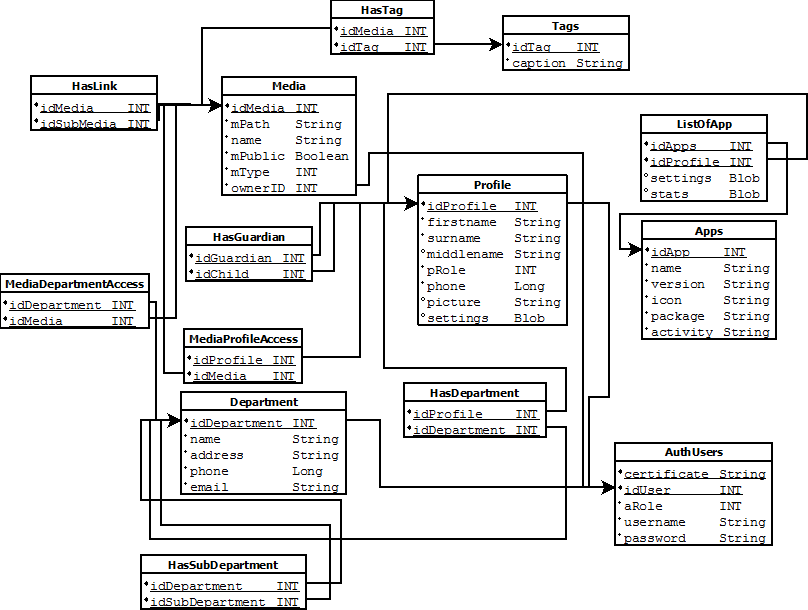
\includegraphics[width=1.00\textwidth]{images/DiaDesign.png}
	\caption{Dia diagram of the database}
	\label{fig:DiaDesign}
\end{figure}

Although the diagram in \autoref{fig:DiaDesign} does not meet the conventions of database diagrams, it does provide a good view of the different tables, and the relations: Foreign keys points to where the value is fetched from.

\subsubsection{Normal Form}
To prevent modification anomalies in the database, it can be normalized. This becomes important when a table is dealing with functional dependencies. The solution is to remove the dependicies from the table to another, e.g. split a table into two new tables. An example of this is shown in \autoref{tab:nonNormalizedExample} and \autoref{tab:NormalizedDatabaseExample}.

\begin{table}[htbp]
	\centering
		\begin{tabular}{|c|c|c|}
		\hline
		 \multicolumn{3}{|c|}{SALES}\\
		\multicolumn{1}{|c}{Customer\_ID} & \multicolumn{1}{c}{Product} & \multicolumn{1}{c|}{Price} \\
		\hline
		1001 & Laundry detergent & 12 \\ \hline
		1007 & Toothpaste & 3 \\ \hline
		1010 & Chlorine bleach & 4 \\ \hline
		1024 & Toothpaste & 3\\	\hline
		\end{tabular}
	\caption{Non-normalized database\cite[p. 114]{sqlForDummies}}
	\label{tab:nonNormalizedExample}
\end{table}

The problem in \autoref{tab:nonNormalizedExample} is that if customer 1001 is removed from the table, not only is his product removed, but the fact that Laundry detergent costs 12\$ is also lost. A way to prevent this, is to split the table into two tables, as seen in \autoref{tab:NormalizedDatabaseExample}

\begin{table}[htbp]
	\centering
		\begin{tabular}{c c}
			\begin{tabular}{|c|c|}
				\hline
		 		\multicolumn{2}{|c|}{CUST\_PURCH} \\
		 		\multicolumn{1}{|c}{Customer\_ID} & \multicolumn{1}{c|}{Product} \\
		 		\hline
		 		1001 & Laundry detergent \\ \hline
		 		1007 & Toothpaste \\ \hline
		 		1010 & Chlorine bleach \\ \hline
		 		1024 & Toothpaste \\ \hline
			\end{tabular}
		&
			\begin{tabular}{|c|c|}
				\hline
				\multicolumn{2}{|c|}{PROD\_PRICE} \\
				\multicolumn{1}{|c}{Product} & \multicolumn{1}{c|}{Price} \\
				\hline
				Laundry detergent & 12 \\ \hline
				Toothpaste & 3 \\ \hline
				Chlorine bleach & 4 \\ \hline
			\end{tabular}
		\end{tabular}
	\caption{Normalized database example\cite[p 115]{sqlForDummies}}
	\label{tab:NormalizedDatabaseExample}
	\end{table}

As seen in \autoref{tab:NormalizedDatabaseExample} the table \code{CUST\_PURCH} now only deals with the customer, and thus it is now possible to remove a customer from the system, without loosing the product's price.

There are several degrees of normal form for a database, here the focus is on the first three: first, second, and third normal form.

\subsubsection{First Normal Form (1NF)}
The example in \autoref{tab:NormalizedDatabaseExample}, is an example of 1NF. To achieve this the following qualities must apply\cite[p. 116]{sqlForDummies}:
\begin{itemize}
	\item Each cell (intersection of a row and a column) of the table must have only a single value.
	\item Each column must have a unique name.
	\item No two rows may be identical (that is, each row must be unique).
	\item Each column contains data for a single attribute of the thing it's describing.
\end{itemize}

As seen in \autoref{fig:DiaDesign} the Savannah database fullfills the qualities of 1NF, and thus is 1NF.

\subsubsection{Second Normal Form (2NF)}
For a database to be in 2NF it is required that if a table contains a composite key, all other attributes in the table must be depended on the entire key.
Furthermore \cite[p. 117]{sqlForDummies} states:
\begin{quotation}
...every
relation that is in 1NF with a single attribute key is automatically in second
normal form.
\end{quotation}
As this is the case in the Savannah database, it is in 2NF.

\subsubsection{Third Normal Form (3NF)}
For a database to be in 3NF, it is required that there are no transitive dependency\footnote{A transitive dependency occurs when one attribute depends on a second
attribute, which depends on a third attribute. Deletions in a table with such a
dependency can cause unwanted information loss. \cite[p. 118]{sqlForDummies}}.
As seen in \autoref{fig:DiaDesign} Savannah's database lives up to this quality, as there are no transitive dependencies within any of the tables. A good example of this is the handling of a profile's access to apps: When the app is removed from the profile it is done in the \code{ListOfApps} table, and thus only the relation is removed, and the specific app is still available in the system. This means the Savannah database is in 3NF.



\subsubsection*{Constraints}
\label{databaseRules}
To provide the security needed in the system, several constraints need to apply for the database:
\begin{itemize}
	\item The \code{Profile}$\rightarrow$\code{AuthUsers} relation must be one-to-one, as one user from the \code{AuthUsers} can only have one profile in the system
	\item The \code{Department}$\rightarrow$\code{AuthUsers} relation must be one-to-one, as one department from the \code{AuthUsers} can only be one department in the system
	\item The \code{idUser} attribute in \code{AuthUsers} must be unique.
	\item The \code{username} attribute in \code{AuthUsers} must be unique
	\item It must be possible to distinguish between users and departments in the \code{AuthUsers} table
	\item It must be possible to distinguish between children, parents and guardians in the \code{Profile} table
\end{itemize}

These constraints will be implemented through the use of SQL scripts and Java code in \textbf{REF TIL SECTION} %TODO